\documentclass[dvipsnames,tikz]{standalone}
\usepackage{amsmath}
\usepackage{arevmath}
\usepackage{xcolor}
\usepackage{tikz}
\usetikzlibrary{calc}
\usetikzlibrary{decorations.pathreplacing,calligraphy,3d}
\usetikzlibrary{lindenmayersystems}

\tikzset{main/.style={draw=black, circle, color=black}}

\begin{document}
	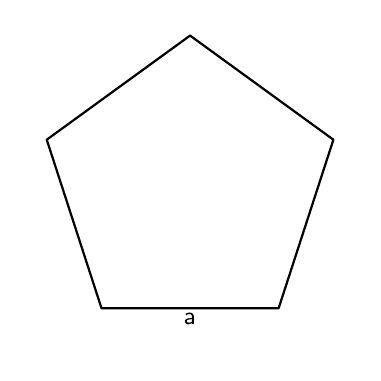
\begin{tikzpicture}[scale=0.75, main, line join=bevel]
		\clip(-1.25,-0.75) rectangle (4.25,4.75);
		\draw (1.5,0) node [below, yshift=4pt] {\small \textsf{a}};
		\draw [thick, main] (0,0)-- (3,0) -- (3.927,2.853) -- (1.5,4.616) -- (-0.927,2.853) -- cycle;
	\end{tikzpicture}
	
	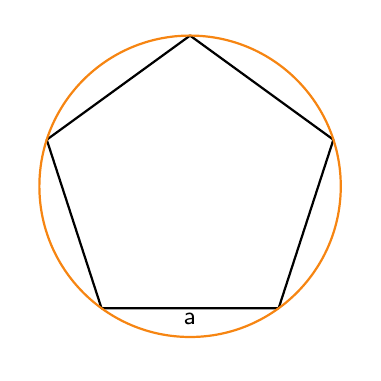
\begin{tikzpicture}[scale=0.75, main, line join=bevel]
		\clip(-1.25,-0.75) rectangle (4.25,4.75);
		\draw (1.5,0) node [below, yshift=4pt] {\small \textsf{a}};
		\draw [thick, main] (0,0)-- (3,0) -- (3.927,2.853) -- (1.5,4.616) -- (-0.927,2.853) -- cycle;
		\draw [thick, main, BurntOrange] (1.5,2.064) circle (2.5519cm);
	\end{tikzpicture}
	
	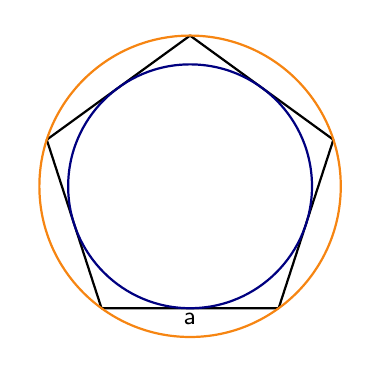
\begin{tikzpicture}[scale=0.75, main, line join=bevel]
		\clip(-1.25,-0.75) rectangle (4.25,4.75);
		\draw (1.5,0) node [below, yshift=4pt] {\small \textsf{a}};
		\draw [thick, main] (0,0)-- (3,0) -- (3.927,2.853) -- (1.5,4.616) -- (-0.927,2.853) -- cycle;
		\draw [thick, main, BurntOrange] (1.5,2.064) circle (2.5519cm);
		\draw [thick, main, NavyBlue] (1.5,2.064) circle (2.0645cm);
		
	\end{tikzpicture}
	
	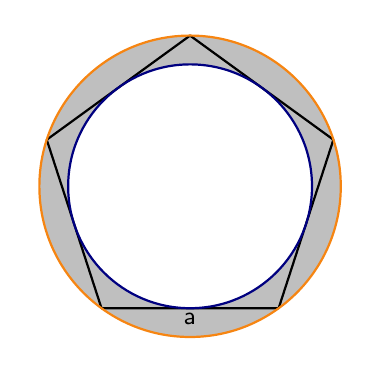
\begin{tikzpicture}[scale=0.75, main, line join=bevel]
		\clip(-1.25,-0.75) rectangle (4.25,4.75);
		\fill[gray, semitransparent,even odd rule] (1.5,2.064) circle (2.5519cm) (1.5,2.064) circle (2.0645cm);
		\draw (1.5,0) node [below, yshift=4pt] {\small \textsf{a}};
		\draw [thick, main] (0,0)-- (3,0) -- (3.927,2.853) -- (1.5,4.616) -- (-0.927,2.853) -- cycle;
		\draw [thick, main, BurntOrange] (1.5,2.064) circle (2.5519cm);
		\draw [thick, main, NavyBlue] (1.5,2.064) circle (2.0645cm);
	\end{tikzpicture}
\end{document}